\documentclass[10pt]{article}
% ---------------------------------------------------------------
% One-page complete summary of the DTW+S paper
%   A. Srivastava, "DTW+S: Shape-based Comparison of Time-series
%   with Ordered Local Trends", arXiv:2309.03579 (v3, Dec 2024);
%   published at AAAI 2025 as "Aligning time-series by local
%   trends: Applications in public health".
% ---------------------------------------------------------------
\usepackage[margin=0.75in]{geometry}
\usepackage{amsmath,amssymb}
\usepackage{enumitem}
\usepackage{graphicx}
\usepackage{float}
\usepackage{xcolor}
\usepackage[colorlinks=true,linkcolor=blue,urlcolor=blue]{hyperref}
\setlist{nosep,leftmargin=*}
\setlength{\parskip}{2pt}
\setlength{\parindent}{0pt}
\pagestyle{empty}

\newcommand{\head}[1]{\smallskip\noindent\textbf{#1}\quad}

\begin{document}
{\large\textbf{DTW+S: Shape-based Comparison of Time-series with Ordered Local Trends --- a complete summary}}\\[2pt]
{\small Ajitesh Srivastava (USC). arXiv:2309.03579v3 (Dec.\ 2024); published at AAAI~2025 as
``Aligning time-series by local trends: Applications in public health''.
\href{https://arxiv.org/abs/2309.03579}{arxiv.org/abs/2309.03579}}

\head{Problem.} Standard distances (Euclidean / MAE, correlation, plain DTW) can rank a flat,
information-free line as \emph{closer} to a ground-truth curve than a forecast that reproduces
the right shape but is slightly off in height or time. The author wants a distance for which two
series are similar \emph{iff} they show a \emph{similar sequence of local trends occurring around
similar times}, scale-tolerant, and --- crucially --- \emph{interpretable} for applied users
(epidemiologists), who resist black-box metrics. Target setting: series with \emph{ordered local
trends} (e.g.\ epidemics: surge $\to$ increase $\to$ peak $\to$ decrease).

\head{Core idea.} Two stages. (1) Transform each series into an interpretable
\emph{Shapelet-Space Representation} (SSR): slide a window of length $w$ over the series and, at
each position, map the window to a $d$-dimensional vector of similarities to pre-chosen
\emph{shapelets} (shapes of interest). This yields a matrix $A\in\mathbb{R}^{d\times(T-w+1)}$ whose
columns are interpretable local trends over time. (2) Apply \emph{DTW} between the SSR matrices of
two series, using squared Euclidean distance between columns $\lVert A[:,i]-B[:,j]\rVert^2$, so that
similar trends are matched even if shifted in time (warping window $\tau$; e.g.\ $\tau=5$ weeks for
epidemics, a tuned hyper-parameter for classification). Distance $=$ DTW on shapes $=$ \textbf{DTW+S}.

\head{Shapelet space \& closeness preservation.} Shapelets are fixed domain shapes (used throughout:
\texttt{increase}=[1,2,3,4], \texttt{surge}=[1,2,4,8], \texttt{peak}=[1,2,2,1], \texttt{flat}=[0,0,0,0]).
Each coordinate is a (flatness-gated) correlation of the normalized window to a shapelet; an explicit
``flatness'' factor stops noisy near-flat windows from looking like real shapes. The design enforces
\emph{Closeness Preservation}: two windows get similar representations iff one is a scale/translation of
the other, or both are ``almost flat''.

\begin{figure}[H]
\centering
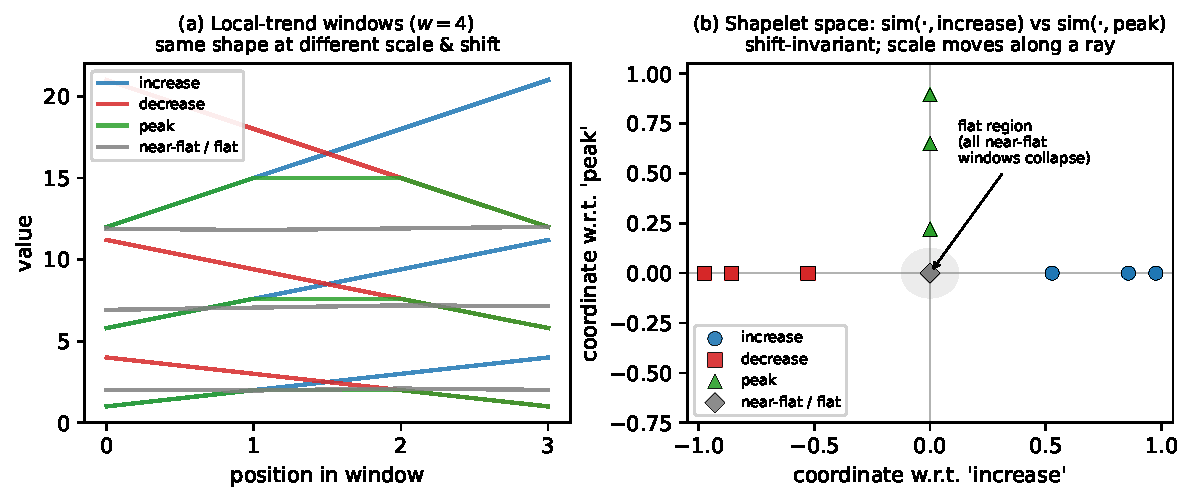
\includegraphics[width=0.92\textwidth]{fig_shapelet_space.pdf}
\caption{Closeness preservation, computed with the paper's formulas (shapelets
\texttt{increase}/\texttt{peak}; coordinate $\mathrm{sim}(x,s_i)=(1-\gamma)\,\mathrm{corr}(x,s_i)$).
\textbf{(a)} Length-4 windows of the same shape at different scales and time-shifts.
\textbf{(b)} Their shapelet-space coordinates: \emph{translation-invariant} (shifted copies overlap),
shape sets the \emph{direction} (increases on $+x$, decreases on $-x$, peaks on $+y$), and amplitude
moves a window \emph{along a ray}; every ``almost-flat'' window --- whatever its underlying shape ---
collapses into the shaded flat region at the origin. This is exactly Property~1: similar representation
$\iff$ (i) one is a scale/translation of the other, or (ii) both are almost flat.}
\end{figure}

\head{Theory.} (1) \emph{Theorem 1+2:} exactly $w-1$ linearly independent shapelets plus the flat
shapelet are \emph{necessary and sufficient} to satisfy closeness preservation. (2) \emph{Theorem 3
(expressive power):} a proper shapelet-space transform can discriminate \emph{any} trend descriptor
(including, via the flat dimension, some scale information) --- unlike finite-label encoders that
collapse distinct shapes (e.g.\ ``peak'' vs ``increase'').

\head{Ensembling (a key contribution).} \emph{Setting:} several models each forecast the same
epidemic, and we want one ``consensus'' curve. The usual method (a \emph{mean ensemble}) just averages
the curves \emph{vertically} --- at each week, take the average of the values. This misleads when the
peaks don't line up in time. Example: model~A peaks at week~10 and model~B at week~14, each reaching
1000 cases. Averaging week-by-week gives no sharp peak --- only a lower, wider bump around week~12 that
\emph{neither} model predicted, making the wave look far milder than both forecasts say. DTW+S fixes
this by averaging \emph{matching events} instead of fixed clock-times: it first uses the shape
alignment to see that A's peak and B's peak are \emph{the same event}, then averages their \emph{timing}
(weeks 10 and 14 $\to$ week~12) \emph{and} their \emph{height} (1000 and 1000 $\to$ 1000). The consensus
curve then keeps a real peak of $\sim$1000 at week~12. \emph{How it is computed} (\emph{DTW+S Barycenter
Averaging}, Alg.~2): pick one curve as a starting reference, align every curve to it with DTW+S and
average to get an updated reference, and repeat until the reference stops changing.

\head{Clustering \& classification.} The DTW+S distance plugs into any distance-based method: the
paper uses agglomerative clustering (number of clusters via Silhouette) and 1-nearest-neighbor
classification (chosen so the distance measure alone decides the label).

\head{Experiments \& results.} (1) \emph{Ensemble:} on 12 synthetic peak sets, DTW+S~BA cuts
fractional error in recovered peak \emph{size and timing} to $\approx$0.01--0.03, vs.\ $\approx$0.1--0.4
for mean / plain-DTW / z-normalized-DTW ensembles. (2) \emph{Clustering:} gives more sensible groupings
of epidemic curves than DTW or SSR alone. (3) \emph{Classification (UCR archive, 1-NN):} DTW+S beats
plain DTW on a large subset of the 64 datasets where local trends (not scale) are decisive, and beats
shapeDTW on nearly half; light pre-smoothing (tuned) further improves many datasets. (4)
\emph{Interpretability:} SSR heat-maps directly reveal \emph{why} two series differ (e.g.\ a bright
``peak'' dimension around $t\!=\!25$ separating two classes).

\head{Relation to prior work.} Closest is shapeDTW (point-wise shape descriptors); DTW+S instead uses
\emph{interpretable, domain-chosen} shapelets with provable closeness-preservation guarantees, and is
purpose-built for ordered-trend / epidemic applications rather than general use.

\head{Limitations.} Not meant for general-purpose tasks where scale dominates shape; best use needs
domain knowledge to choose shapelets and set warping/smoothing parameters (Theorems 1--2 only guide the
shapelet choice); current DTW step is $O(T^2)$ time and space (speed-ups left to future work). Notably,
evaluation is entirely \emph{computational} (ensembling / clustering / classification) --- there is
\emph{no human-perception study} of whether its alignments match how people judge similarity.
\end{document}
